\documentclass[11pt]{article}

\usepackage{amsmath}
\usepackage[margin=0.68in]{geometry}
\usepackage{booktabs}
\usepackage{enumitem}
\usepackage{fancyhdr}
\usepackage{graphicx}
\usepackage[hidelinks]{hyperref}
\usepackage{listings}
\usepackage{microtype}
\usepackage{tabularx}
\usepackage{tikz}
\usepackage{titlesec}
\usepackage[table]{xcolor}
\usetikzlibrary{arrows.meta,positioning}
\graphicspath{{docs/lessons/assets/}{../assets/}}

\definecolor{AdkBlack}{gray}{0}
\definecolor{AdkDark}{gray}{0.20}
\definecolor{CodeGray}{gray}{0.96}
\hypersetup
{
    pdftitle={ADK Lesson 014: Character Display and Stable Records},
    pdfauthor={Kevin Shanahan},
    pdfsubject={Owned HD44780 presentation, incremental updates, and locale-independent climate records},
    pdflang={en-US}
}
\pagestyle{fancy}
\fancyhf{}
\lhead{\textsc{ADK Lesson 014}}
\rhead{Character Display and Stable Records}
\cfoot{\thepage}
\setlength{\headheight}{14pt}
\setlength{\parindent}{0pt}
\setlength{\parskip}{5pt}
\setlist{nosep,leftmargin=1.45em}
\titleformat{\section}{\Large\bfseries\color{AdkBlack}}{\thesection}{0.5em}{}
\titleformat{\subsection}{\large\bfseries\color{AdkBlack}}{\thesubsection}{0.5em}{}
\lstdefinestyle{adkcpp}
{
    language=C++,
    backgroundcolor=\color{CodeGray},
    basicstyle=\ttfamily\footnotesize,
    keywordstyle=\color{AdkBlack}\bfseries,
    commentstyle=\color{AdkDark},
    columns=fullflexible,
    keepspaces=true,
    showstringspaces=false,
    frame=single,
    rulecolor=\color{black!20},
    breaklines=true,
    tabsize=4
}
\newcommand{\checkbox}{\(\square\)}
\newcommand{\blank}[1]{\rule{#1}{0.4pt}}
\newcommand{\warningbox}[1]{%
  \begin{center}
  \fcolorbox{black}{white}{\parbox{0.91\linewidth}{\textbf{Safety checkpoint.} #1}}
  \end{center}}
\newcommand{\evidencebox}[1]{%
  \begin{center}
  \fcolorbox{black}{white}{\parbox{0.91\linewidth}{#1}}
  \end{center}}

\begin{document}

\begin{center}
  {\Huge\bfseries Character Display and Stable Records}\\[4pt]
  {\Large Keep state, presentation, transport, and evidence separate}\\[8pt]
  \textit{The display shows meaning; TP14 shows transport; the record preserves facts.}
\end{center}

\begin{tabularx}{\linewidth}{@{}>{\bfseries}l X >{\bfseries}l X@{}}
Lesson & 014 --- component & Time & 120--180 minutes\\
Prerequisites & Lessons 001--013 & Board & Arduino Mega 2560\\
Evidence & D13 acquisition, LCD text, TP14 enable & Status &
host verified; physical acceptance open\\
Safety & E1; USB-powered low-current circuit only\\
\end{tabularx}

\warningbox{Disconnect USB before wiring. Identify the exact LCD module and
its pin order from primary documentation. Do not assume its backlight includes
a resistor. If the backlight current limit or polarity is unknown, leave pins
A and K disconnected. Stop for heat, odor, resets, unstable power, a contrast
control that places a rail across the potentiometer wiper incorrectly, or any
disagreement between the identified module and the literal table. Remove USB
power to stop the experiment.}

\section{Mission}

Present a deterministic climate snapshot without making the display the source
of truth:

\[
\texttt{ClimateSample}\rightarrow
\left\{
\begin{array}{ll}
\texttt{Hd44780Display} & \text{short human view}\\
\texttt{formatClimateRecord()} & \text{stable machine record}
\end{array}
\right.
\]

The canonical sketch replays four fixed samples. This isolates presentation
from sensing: the same sample selects both LCD text and a record, while neither
path modifies the sample. Lesson 015 will replace the fixed table with the
scheduled sensor from lesson 013.

\begin{enumerate}
  \item Predict the first two lines and the next sequence number.
  \item Observe D13 before expecting text, then observe the LCD update.
  \item Observe TP14 only as transport evidence.
  \item Interpret the record and display as two views of one immutable sample.
\end{enumerate}

\section{The four boundaries}

\begin{center}
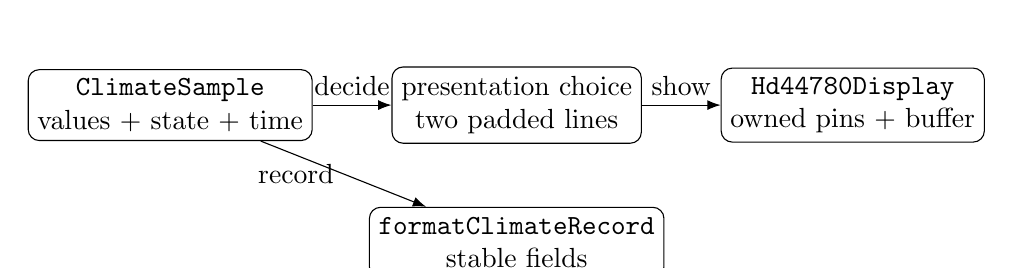
\begin{tikzpicture}[
    node distance=8mm and 10mm,
    box/.style={draw,rounded corners,minimum height=9mm,align=center},
    >=Latex]
  \node[box] (state) {\texttt{ClimateSample}\\values + state + time};
  \node[box,right=of state] (present) {presentation choice\\two padded lines};
  \node[box,right=of present] (lcd) {\texttt{Hd44780Display}\\owned pins + buffer};
  \node[box,below=of present] (record) {\texttt{formatClimateRecord}\\stable fields};
  \draw[->] (state) -- node[above]{decide} (present);
  \draw[->] (present) -- node[above]{show} (lcd);
  \draw[->] (state) -- node[left]{record} (record);
\end{tikzpicture}
\end{center}

\texttt{CharacterDisplay} is the substitutable presentation boundary. It
defines lifecycle, caller-driven \texttt{update(now)}, readiness, two-row
\texttt{show()}, and a desired-line snapshot. \texttt{Hd44780Display} is the
concrete 16-by-2, four-bit adapter. It owns RS, E, and D4--D7 through six fixed
resource claims.

Construction is inert. \texttt{initialize()} validates distinct Mega digital
pins, acquires all six before exposing behavior, configures them low, and
starts a staged power-up sequence. A conflict or injected configuration
failure releases every claim. Repeated initialization is inert.

\texttt{update(now)} advances at most one startup stage or one changed
character. The caller supplies time; no background task or global callback
exists. The bounded one-microsecond enable pulse is an electrical transport
operation, not an application schedule. \texttt{shutdown()} commands display
off when possible, drives owned pins low, releases them to high impedance, and
is idempotent. Destruction repeats this safely.

\section{Parts and orientation}

\begin{tabularx}{\linewidth}{@{}l l X@{}}
\toprule
Quantity & Part & Requirement\\
\midrule
1 & Mega 2560 & USB powered\\
1 & HD44780-compatible 16-by-2 LCD & exact module and pin order identified\\
1 & 10\,k\(\Omega\) linear potentiometer & contrast control only\\
1 & backlight resistor & only if required by the identified module data\\
1 & D13 indicator & built-in LED or external resistor-limited LED\\
1 & multimeter & continuity and released-state checks\\
1 & logic analyzer or oscilloscope & optional TP14 enable-pulse evidence\\
\bottomrule
\end{tabularx}

\begin{figure}[ht]
  \centering
  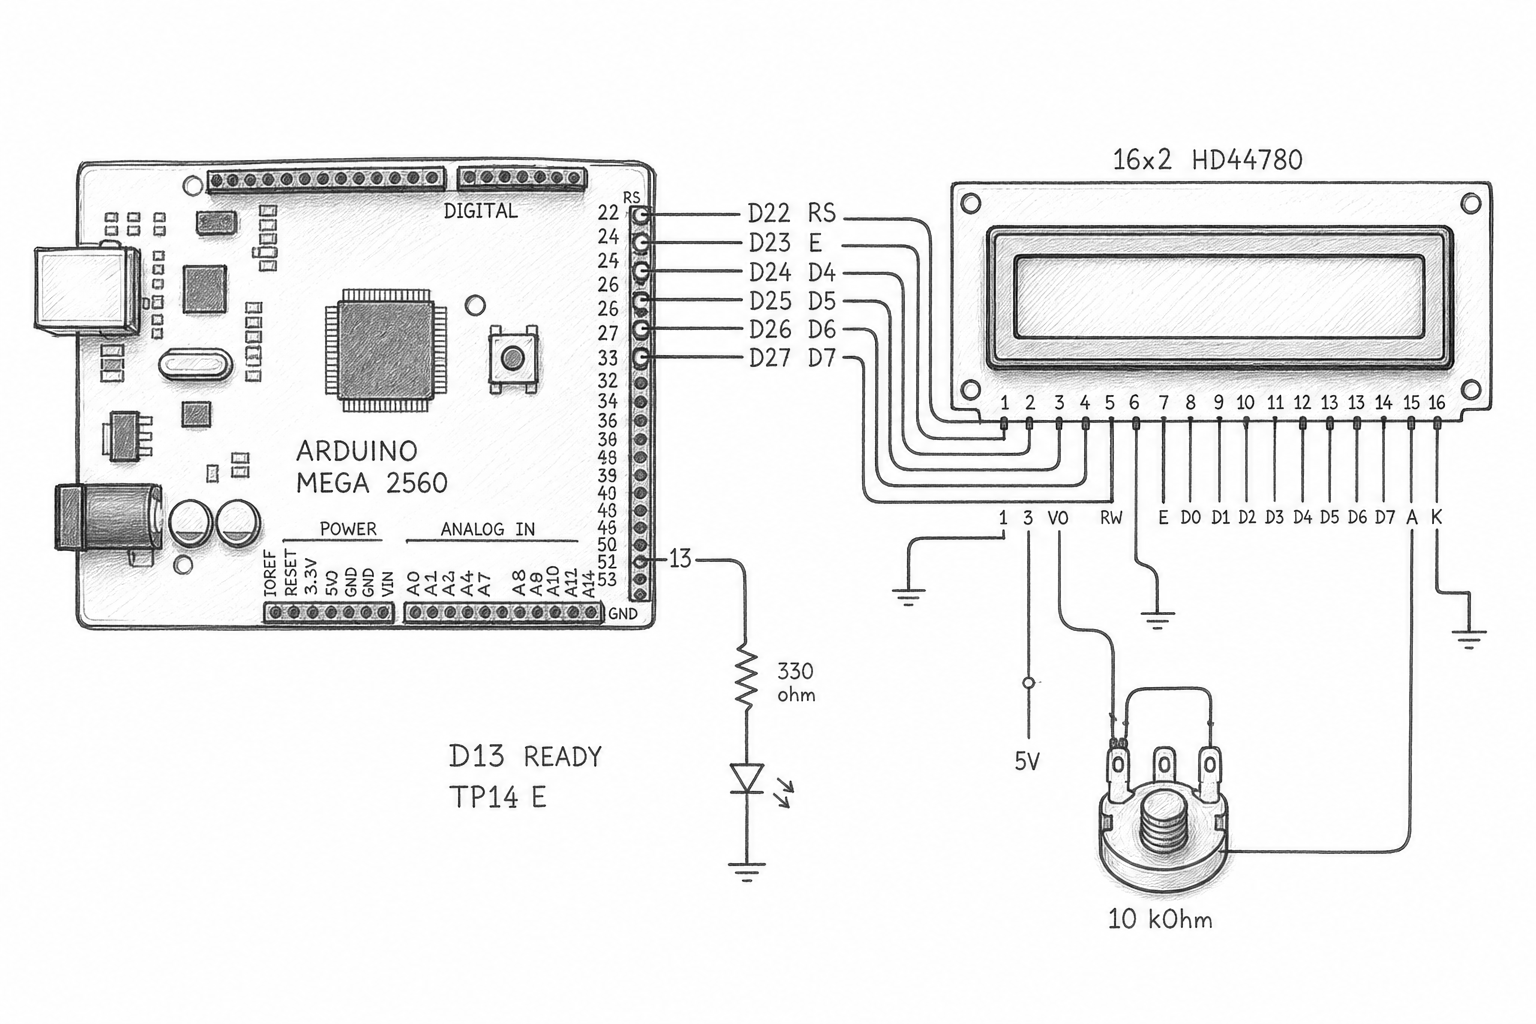
\includegraphics[width=0.98\linewidth]{014-character-display-pencil.png}
  \caption{Pencil orientation of the Mega, LCD, contrast control, D13 evidence,
  and TP14. This is not an authoritative schematic; some drawn board labels
  are illustrative. Use the literal table and the exact module documentation.
  Alternative text: six Mega signal wires reach LCD RS, E, and D4 through D7;
  RW and VSS return to ground; VDD reaches 5 V; a potentiometer supplies VO;
  D13 separately indicates resource acquisition; TP14 is the E node.}
\end{figure}

\section{Literal wiring}

\begin{tabularx}{\linewidth}{@{}l l X@{}}
\toprule
Function & Mega connection & Literal path\\
\midrule
LCD supply & 5 V and GND & identified VDD to 5 V; VSS to GND; never use Vin\\
contrast & VO & 10 k\(\Omega\) ends to 5 V/GND; wiper to identified VO\\
write policy & RW & identified RW directly to GND\\
register select & D22 & D22 to identified RS\\
enable / TP14 & D23 & D23 to identified E; label this node TP14\\
data bit 4 & D24 & D24 to identified D4\\
data bit 5 & D25 & D25 to identified D5\\
data bit 6 & D26 & D26 to identified D6\\
data bit 7 & D27 & D27 to identified D7\\
unused data & none & D0--D3 remain unconnected in four-bit mode\\
backlight & A and K & connect only per identified module rating and polarity\\
acquisition & D13 & built-in LED, or D13 through 330 \(\Omega\) to LED anode\\
\bottomrule
\end{tabularx}

Inspect every path with USB removed. Set the contrast control near its midpoint
before power. If using an external D13 LED, return its cathode to GND and
record its resistor value. TP14 is measured relative to the same named GND.
Place analyzer clips while unpowered.

\section{Startup and incremental work}

An HD44780 controller is not ready when the MCU resets. The adapter models that
fact explicitly:

\[
\text{claim}\rightarrow15\text{ ms}\rightarrow
3,3,3,2\text{ nibbles}\rightarrow
\text{function, off, clear, entry, on}\rightarrow\text{ready}.
\]

Calls made before \texttt{ready()} only advance startup when their caller time
is due. Once ready, \texttt{show(row,text)} updates the desired 16-character
line. It rejects a null pointer, nonprinting ASCII, an unknown row, or text
longer than 16 characters without touching the LCD.

Each later \texttt{update(now)} compares desired and shown buffers and writes
one changed cell. A loop therefore remains responsive while a whole line
changes. The desired snapshot is stable until another \texttt{show()} call.

\begin{lstlisting}[style=adkcpp]
void loop ()
{
    const adk::TimePoint now (millis ());

    display.update (now);

    if (display.ready () && sampleDue (now))
    {
        const adk::ClimateSample sample = decideSample (now);
        showSample   (sample);
        recordSample (sample);
    }
}
\end{lstlisting}

\section{Stable records}

The record format is ASCII, one line, with fixed field order and explicit
units:

\begin{verbatim}
seq=42,state=valid,temp_centi_c=-125,rh_permille=456,at_ms=4294967290
\end{verbatim}

Integers avoid decimal punctuation and floating-point formatting. Names encode
units. States such as \texttt{transport\_timeout},
\texttt{checksum\_failure}, and \texttt{stale} remain distinct. The timestamp
is the sample observation time, not the time the line happened to print.

\texttt{formatClimateRecord()} allocates nothing and does not use locale. The
caller supplies a buffer. A too-small buffer is terminated and reports
\texttt{CapacityExceeded}; a null or zero-capacity buffer reports
\texttt{InvalidArgument}. Serial output in the canonical sketch merely carries
this record. It is optional evidence: the LCD and TP14 provide the required
non-Serial paths.

\section{Predict, observe, interpret}

\begin{tabularx}{\linewidth}{@{}p{0.19\linewidth} X X@{}}
\toprule
Claim & Prediction and observation & Interpretation\\
\midrule
resource acquisition & D13 turns on after all seven objects' pin claims succeed &
D13 off means setup did not complete; it says nothing about LCD text\\
safe startup & before ready, signal pins start low and the LCD may remain blank &
blank during the specified startup interval is not yet a sensor fault\\
transport & TP14 has bounded enable pulses as cells change &
pulses prove attempted writes, not readable contrast or correct data wiring\\
presentation & fixed samples appear in the documented order &
text order tests the presentation table and incremental flush\\
record identity & sequence increases once per displayed sample &
one sample produced both views; locale cannot alter field punctuation\\
safe shutdown & D13 turns off and D22--D27 become high impedance &
resource release is separate from the last visible LCD pixels\\
\bottomrule
\end{tabularx}

\evidencebox{\textbf{Important distinction.} An LCD can retain visible pixels
after MCU pins become high impedance. That persistence is not evidence that
ADK still owns or drives the pins. Measure the released electrical state at a
named signal pin; use the display only as semantic evidence.}

\section{Host experiments}

Run the registered repository target after integration:

\begin{verbatim}
make host-test
make host-test-sanitize
make arduino-compile
make serial-monitor PORT=/dev/ttyACM0 BAUD=115200
\end{verbatim}

The deterministic tests cover:

\begin{itemize}
  \item stopped, repeated-start, repeated-shutdown, and destructor behavior;
  \item staged startup from supplied timestamps;
  \item invalid rows, null text, nonprinting characters, and capacity limits;
  \item duplicate pins, resource conflict, configuration rollback, and reuse;
  \item one-cell incremental flushing and stable desired-line snapshots;
  \item exact signed values, every state name, maximum timestamps, and small
        record buffers;
  \item injected transport-write failures without hidden retries.
\end{itemize}

Run the same trace twice. Compare the transport operation sequence and record
bytes. Identical inputs must produce identical outputs.

\section{Bench procedure}

\begin{enumerate}
  \item \textbf{Predict.} Write the first line pair and first record below.
  \item Remove USB. Identify the module pin-one mark and backlight rating.
  \item Wire only supply, contrast, RW, and the six signal paths. Leave the
        backlight disconnected unless its current path is known.
  \item Check for shorts from 5 V to GND and verify RW-to-GND continuity.
  \item Place the TP14 and GND clips while unpowered.
  \item Apply USB. Confirm D13 turns on before interpreting LCD behavior.
  \item Adjust contrast slowly. Observe four fixed views in order.
  \item Observe TP14 during changes. Do not infer timing from this drawing;
        record the instrument and measured pulse range.
  \item Invoke or instrument shutdown. Confirm D13 off, then measure one signal
        pin as released rather than inferring release from the retained text.
  \item Remove USB. Confirm the display and D13 are unpowered.
\end{enumerate}

Predicted first view: \blank{0.72\linewidth}

Predicted first record: \blank{0.68\linewidth}

\section{Diagnosis}

\begin{tabularx}{\linewidth}{@{}l X X@{}}
\toprule
Observation & Likely boundary & Next safe check\\
\midrule
D13 remains off & claim or initialization failure & remove power; check distinct D22--D27 wiring and conflicts\\
D13 on, no blocks or text & supply, contrast, or startup & remove power; verify VSS/VDD/VO and module identity\\
blocks but no text & RS/E/data mapping & remove power; compare every literal path\\
wrong characters & D4--D7 order or intermittent connection & remove power; continuity-check each data path\\
TP14 quiet while text queued & loop halted or transport failure & inspect D13 and deterministic host trace\\
TP14 active, unreadable LCD & contrast, supply, or data mapping & do not treat transport as presentation proof\\
record differs by locale & unsupported formatter introduced & compare exact bytes to the stable grammar\\
old pixels after shutdown & normal LCD memory persistence & measure high impedance at a named MCU signal\\
\bottomrule
\end{tabularx}

\section{Exercises}

\begin{enumerate}
  \item Explain why a display object owns pins while a presentation table owns
        no hardware.
  \item Add a fourth record consumer that counts states without parsing LCD
        text. What boundary should it accept?
  \item Calculate the maximum number of loop calls needed to replace both
        16-character lines when one dirty cell flushes per call.
  \item Add a test for \(-32768\) centi-degrees and explain why negation first
        widens to 32 bits.
  \item Design a 20-by-4 extension without changing the climate sample or
        stable-record grammar. Which dimensions become configuration?
  \item Inject a write failure on the enable-low operation. Predict the status,
        desired snapshot, and caller's safe response.
  \item Explain why LCD pixel persistence cannot prove output shutdown.
\end{enumerate}

\section{Acceptance record}

\begin{tabularx}{\linewidth}{@{}l X@{}}
\toprule
Item & Record\\
\midrule
Board and USB supply & \blank{0.63\linewidth}\\
LCD manufacturer/module/revision & \blank{0.54\linewidth}\\
Primary pinout source & \blank{0.62\linewidth}\\
Backlight rating/path, or disconnected & \blank{0.49\linewidth}\\
Contrast potentiometer measured value & \blank{0.49\linewidth}\\
D13 evidence behavior & \blank{0.61\linewidth}\\
TP14 instrument and pulse observation & \blank{0.47\linewidth}\\
Four displayed views in order & \blank{0.57\linewidth}\\
Stable record bytes checked & \blank{0.58\linewidth}\\
Shutdown pin and measured released state & \blank{0.45\linewidth}\\
Reset and power-removal observations & \blank{0.49\linewidth}\\
Deviation, reviewer, date & \blank{0.62\linewidth}\\
\bottomrule
\end{tabularx}

\textbf{Current release statement:} implementation and deterministic host
tests are complete for this package. Mega compilation and size evidence are
recorded by the integrator. Physical behavior, electrical levels, contrast,
backlight current, timing, shutdown, reset, and power removal remain
\textbf{open} until the table above contains measured results.

\section{Next}

Lesson 015 composes the scheduled climate sensor, this character display,
stable records, and explicit health policy into an environmental station. It
does not turn this learning circuit into a calibrated monitor or safety alarm.

\end{document}
